\section{Phương pháp thực hiện}

Phần này trình bày chi tiết các phương pháp kỹ thuật và kiến trúc mô hình được triển khai trong hệ thống phân tích hợp đồng pháp lý. Hệ thống được xây dựng theo mô hình pipeline tuần tự, trong đó đầu ra của các tác vụ xử lý cú pháp ở tầng thấp (Assignment 1) sẽ là tiền đề và đặc trưng đầu vào cho các mô hình trích xuất ngữ nghĩa ở tầng cao (Assignment 2). Cuối cùng, toàn bộ tri thức có cấu trúc được tích hợp vào hệ thống RAG (Assignment 3) để phục vụ hỏi đáp.

Điểm đặc trưng trong phương pháp thực hiện của đồ án là việc sử dụng kỹ thuật \textit{Multi-Sample Dropout} \autocite{multidrop} kết hợp với kiến trúc PhoBERT để tăng cường khả năng chống nhiễu đối với các biến thể ngôn ngữ pháp lý, đồng thời áp dụng cơ chế \textit{Sequence Labeling} để giải quyết bài toán tách mệnh đề phức tạp thay vì các phương pháp sinh văn bản (Generative) truyền thống vốn dễ gây hiện tượng ảo giác thông tin.

\subsection{Phân tích Cú pháp (Assignment 1)}

Mục tiêu của giai đoạn này là chuyển đổi văn bản thô từ các dòng văn bản đơn lẻ thành một cấu trúc có phân cấp cú pháp rõ ràng, bao gồm việc xác định ranh giới các mệnh đề logic, nhận diện các cụm danh từ và xây dựng cây quan hệ ngữ pháp.

\subsubsection{Tách mệnh đề (Clause Segmentation)}

Văn bản pháp lý thường chứa các câu phức với cấu trúc phân phối (ví dụ: một chủ ngữ thực hiện nhiều hành động hoặc một hành động áp dụng cho nhiều đối tượng). Để trích xuất thông tin chính xác, hệ thống cần phân rã các câu này thành các mệnh đề độc lập.

\paragraph{Kiến trúc mô hình:}
Hệ thống sử dụng mô hình \texttt{RobustSegmenterModel} dựa trên PhoBERT. Thay vì dự đoán vị trí ngắt câu đơn thuần, mô hình được huấn luyện để gán nhãn cho từng token theo 5 nhóm thành phần (từ 1 đến 5). Tùy thuộc vào cấu trúc của câu phức, ngữ nghĩa và vai trò của các khối này được phân định thành 2 trường hợp (Type) rõ rệt:

\begin{itemize}
    \item \textbf{Type 1 (Cấu trúc phân phối nhánh song song):} Dùng cho các câu có chung phần mở đầu và kết thúc, nhưng phân nhánh ở giữa.
    \begin{itemize}
        \item \textbf{1 (A)}: Phần mở đầu chung (thường là chủ ngữ hoặc mệnh đề dẫn).
        \item \textbf{2 (B)}: Nhánh nội dung thứ nhất.
        \item \textbf{3 (C)}: Nhánh nội dung thứ hai.
        \item \textbf{4 (D)}: Phần kết thúc / bổ ngữ chung.
        \item \textbf{5 (E)}: \textit{Không sử dụng (Trống).}
    \end{itemize}
    \item \textbf{Type 2 (Cấu trúc phân phối vị ngữ dùng chung tân ngữ):} Dùng cho các câu có hai vị ngữ cùng tác động lên một tân ngữ chung, nhưng vị ngữ thứ hai có thêm phần bổ ngữ kéo theo.
    \begin{itemize}
        \item \textbf{1 (A)}: Chủ ngữ chung.
        \item \textbf{2 (B)}: Vị ngữ thứ nhất.
        \item \textbf{3 (C)}: Tân ngữ chung.
        \item \textbf{4 (D)}: Vị ngữ thứ hai.
        \item \textbf{5 (E)}: Bổ ngữ riêng của vị ngữ thứ hai.
    \end{itemize}
\end{itemize}

\paragraph{Thuật toán tái tổ hợp (Reconstruction Algorithm):}
Dựa trên sự hiện diện của khối 5 (E), hệ thống sẽ quyết định logic lắp ghép lại câu để tạo ra các mệnh đề hoàn chỉnh mang đầy đủ ngữ nghĩa.

\begin{verbatim}
Algorithm: Clause Reconstruction
Input: Predicted token labels (1 to 5) and original text
Output: List of independent clauses

1. Group tokens into blocks b1, b2, b3, b4, b5 based on labels
2. If b3 and b4 are empty:
       Output = [Original Sentence]
3. Else If b5 is not empty (Type 2 Structure Detected):
       Clause1 = b1 + " " + b2 + " " + b3
       Clause2 = b1 + " " + b4 + " " + b3 + " " + b5
       Output = [Clause1, Clause2]
4. Else (Type 1 Structure Detected):
       Clause1 = b1 + " " + b2 + " " + b4
       Clause2 = b1 + " " + b3 + " " + b4
       Output = [Clause1, Clause2]
5. Clean up redundant spaces and enforce trailing periods.
\end{verbatim}

Điểm đặc biệt trong file \texttt{src/preprocessing/segmenter.py} là việc sử dụng \texttt{idx\_map} để ánh xạ ngược từ token của PhoBERT về index ký tự trong văn bản gốc, đảm bảo các mệnh đề sau khi tách không bị mất dấu câu hoặc sai lệch định dạng.

\paragraph{Ví dụ minh họa tiến trình tách câu:}
Dưới đây là minh họa quá trình hệ thống trích xuất và lắp ghép cho cả hai loại cấu trúc trên.

\textbf{Ví dụ Type 1:}
\begin{itemize}
    \item \textbf{Câu gốc:} "Ông An có nghĩa vụ cung cấp tài liệu và bàn giao công cụ cho bà Lan."
    \item \textbf{Gán nhãn khối:} [Ông An có nghĩa vụ]\textsubscript{1} [cung cấp tài liệu]\textsubscript{2} [bàn giao công cụ]\textsubscript{3} [cho bà Lan]\textsubscript{4}.
    \item \textbf{Kết quả:}
    \begin{itemize}
        \item Câu 1 (1+2+4): "Ông An có nghĩa vụ cung cấp tài liệu cho bà Lan."
        \item Câu 2 (1+3+4): "Ông An có nghĩa vụ bàn giao công cụ cho bà Lan."
    \end{itemize}
\end{itemize}

\textbf{Ví dụ Type 2:}
\begin{itemize}
    \item \textbf{Câu gốc:} "Bên A chỉ được đọc bản sao và không được sử dụng vào mục đích khác."
    \item \textbf{Gán nhãn khối:} [Bên A]\textsubscript{1} [chỉ được đọc]\textsubscript{2} [bản sao]\textsubscript{3} [không được sử dụng]\textsubscript{4} [vào mục đích khác]\textsubscript{5}.
    \item \textbf{Kết quả:}
    \begin{itemize}
        \item Câu 1 (1+2+3): "Bên A chỉ được đọc bản sao."
        \item Câu 2 (1+4+3+5): "Bên A không được sử dụng bản sao vào mục đích khác."
    \end{itemize}
\end{itemize}

\subsubsection{Phân cụm danh từ (Noun Phrase Chunking)}

Tác vụ này xác định ranh giới của các cụm danh từ (NP), vốn là các thực thể quan trọng trong hợp đồng.

\paragraph{Phương pháp thực hiện:}
Thay vì sử dụng các bộ luật (Rule-based) dựa trên Part-of-Speech (POS) thường gây sai sót trong tiếng Việt, hệ thống tận dụng trực tiếp kết quả từ mô hình \textit{NER} tại file \texttt{src/preprocessing/chunker.py}. Điểm đắt giá của phương pháp này là sự hợp nhất khéo léo giữa bài toán NER và NP Chunking: ngoài các thực thể pháp lý đặc thù (như PARTY, MONEY, DATE, LAW...), lược đồ NER được thiết kế mở rộng thêm một thực thể bao trùm là \texttt{OBJECT}, nghĩa là mỗi cụm danh từ còn lại trong câu sẽ được gắn nhãn là OBJECT. Nhờ đó, mô hình có thể trích xuất toàn vẹn các cụm danh từ có ý nghĩa chỉ qua một lần quét suy diễn (inference) duy nhất mà không cần phụ thuộc vào trình gán nhãn từ loại (POS Tagger).

\paragraph{Quy trình xử lý:}
\begin{enumerate}
    \item \textbf{Tạo mặt nạ ký tự (Character Mask):} Hệ thống lấy tất cả các thực thể được nhận diện bởi mô hình NER (bao gồm cả \texttt{OBJECT}, chỉ loại trừ nhãn \texttt{PREDICATE} là động từ).
    \item \textbf{Gán nhãn mặt nạ:} Các vị trí ký tự thuộc thực thể được đánh dấu là 1 (Bắt đầu) hoặc 2 (Bên trong).
    \item \textbf{Hợp nhất cụm liền kề:} Nếu giữa hai thực thể chỉ có khoảng trắng, thuật toán sẽ tự động nối chúng thành một cụm danh từ duy nhất để đảm bảo tính toàn vẹn về mặt ngữ nghĩa pháp lý (ví dụ: "Công ty" và "ABC" thành "Công ty ABC").
    \item \textbf{Tokenization:} Sử dụng Regex chuyên dụng để tách từ nhưng vẫn giữ được sự tương quan với mặt nạ ký tự đã tạo.
\end{enumerate}

\paragraph{Định dạng đầu ra:} Sử dụng lược đồ IOB (\textit{Inside, Outside, Beginning}).
\begin{verbatim}
Ví dụ: "Bên thuê thanh toán tiền cọc."
Bên         B-NP
thuê        I-NP
thanh toán  O
tiền        B-NP
cọc         I-NP
.           O
\end{verbatim}

\subsubsection{Phân tích cú pháp phụ thuộc (Dependency Parsing)}

Phân tích phụ thuộc (Dependency Parsing) là quá trình xác định cấu trúc ngữ pháp của mệnh đề bằng cách thiết lập các mối quan hệ định hướng (directed relations) giữa các từ. Việc này giúp chuyển đổi một chuỗi từ tuyến tính (flat text) thành một đồ thị cây có hướng (dependency tree), làm bộc lộ rõ từ nào là trung tâm (Head) và từ nào là phụ thuộc (Dependent). Trong miền dữ liệu hợp đồng pháp lý, việc nắm bắt cấu trúc này đóng vai trò then chốt để xác định ai là chủ thể thực hiện hành động, hành động đó tác động lên đối tượng nào, và trong giới hạn thời gian nào.

\paragraph{Công cụ và Cấu hình:}
Hệ thống tích hợp thư viện \texttt{Stanza} với mô hình ngôn ngữ tiếng Việt (\texttt{vi}). Để tối ưu hóa hiệu năng xử lý hàng loạt và đảm bảo tính ổn định trong môi trường thực thi cục bộ (tránh các lỗi do chứng chỉ SSL hoặc kết nối mạng chập chờn), pipeline của Stanza được tinh chỉnh chạy ở chế độ Offline hoàn toàn thông qua cờ \texttt{DownloadMethod.REUSE\_RESOURCES} tại tệp \texttt{src/preprocessing/parser.py}.

\paragraph{Cơ chế làm phẳng đồ thị (Graph Flattening):}
Các mô hình học sâu ở giai đoạn sau (như PhoBERT cho SRL) không trực tiếp tiêu thụ được cấu trúc đồ thị cây. Do đó, hệ thống thực hiện duyệt qua cây cú pháp do Stanza sinh ra và "làm phẳng" (flatten) nó thành một danh sách (array) các đối tượng JSON tuần tự. Mỗi đối tượng đại diện cho một token với các trường thông tin không gian chi tiết:
\begin{itemize}
    \item \textbf{id}: Index của từ trong mệnh đề (bắt đầu từ 1).
    \item \textbf{token}: Văn bản gốc của từ (đã được nối lại từ các sub-words nếu có).
    \item \textbf{head\_index}: Index của từ cha quản lý từ hiện tại. Nếu từ đó là động từ chính hoặc trung tâm của câu, giá trị này bằng 0.
    \item \textbf{head\_token}: Văn bản của từ cha tương ứng (nhằm phục vụ việc đối chiếu trực quan).
    \item \textbf{relation}: Nhãn quan hệ ngữ pháp phổ quát (Universal Dependencies - UD) như \textit{nsubj} (chủ ngữ danh từ), \textit{obl} (bổ ngữ gián tiếp), \textit{amod} (tính từ bổ nghĩa), v.v.
\end{itemize}

\paragraph{Ví dụ minh họa cấu trúc dữ liệu:}
Dưới đây là một mẫu dữ liệu JSON được hệ thống trích xuất tự động cho mệnh đề: \textit{"Kiểm tra chất lượng hàng hóa khi nhận."}

\begin{verbatim}
{
    "clause": "Kiểm tra chất lượng hàng hóa khi nhận.",
    "dependencies": [
        {
            "id": 1,
            "token": "Kiểm tra",
            "head_index": 0,
            "head_token": "ROOT",
            "relation": "root"
        },
        {
            "id": 2,
            "token": "chất lượng",
            "head_index": 1,
            "head_token": "Kiểm tra",
            "relation": "obj"
        },
        {
            "id": 3,
            "token": "hàng hóa",
            "head_index": 2,
            "head_token": "chất lượng",
            "relation": "nmod"
        },
        {
            "id": 4,
            "token": "khi",
            "head_index": 1,
            "head_token": "Kiểm tra",
            "relation": "obl:tmod"
        },
        {
            "id": 5,
            "token": "nhận",
            "head_index": 4,
            "head_token": "khi",
            "relation": "compound:vmod"
        },
        {
            "id": 6,
            "token": ".",
            "head_index": 1,
            "head_token": "Kiểm tra",
            "relation": "punct"
        }
    ]
}
\end{verbatim}

\paragraph{Phân tích ý nghĩa ngữ liệu:}
Nhìn vào cấu trúc JSON trên, thuật toán ở Assignment 2 (Semantic Role Labeling) có thể dễ dàng nội suy ra logic hành động của câu thông qua các liên kết phụ thuộc mà không cần phân tích ngữ nghĩa quá sâu:
\begin{enumerate}
    \item Động từ trung tâm của câu (đóng vai trò vị ngữ chính) là cụm \texttt{"Kiểm tra"} (\texttt{id: 1}, mang nhãn \texttt{root}).
    \item Đối tượng trực tiếp chịu tác động của hành động kiểm tra (tân ngữ) là \texttt{"chất lượng"} (\texttt{id: 2}, mang nhãn \texttt{obj} phụ thuộc trực tiếp vào \texttt{id: 1}). Đối tượng này được làm rõ ngữ nghĩa hơn bởi cụm \texttt{"hàng hóa"} (\texttt{id: 3}, mang nhãn danh từ bổ nghĩa \texttt{nmod} phụ thuộc vào \texttt{id: 2}).
    \item Mốc thời gian hoặc điều kiện thực hiện hành động được neo vào từ \texttt{"khi"} (\texttt{id: 4}, mang nhãn bổ ngữ chỉ thời gian \texttt{obl:tmod} phụ thuộc trực tiếp vào động từ chính \texttt{id: 1}), kết hợp với động từ phụ \texttt{"nhận"} (\texttt{id: 5}, mang nhãn \texttt{compound:vmod} phụ thuộc vào \texttt{id: 4}).
\end{enumerate}

Cấu trúc JSON phẳng này sau đó sẽ được sử dụng để tạo ra các ma trận ánh xạ (mapping matrix) \texttt{dep\_ids} và \texttt{p\_ner\_ids} (Nhãn NER của từ cha), đóng vai trò là Nhúng Cấu trúc (Structural Embeddings) được nối (concatenate) trực tiếp vào đầu ra của PhoBERT trong bài toán nhận diện vai trò ngữ nghĩa (SRL) ở Tác vụ 2.2.

\subsection{Trích xuất Thông tin và Ngữ nghĩa (Assignment 2)}

Giai đoạn này tập trung vào việc hiểu nội dung chi tiết của từng mệnh đề sau khi đã được phân tách ở Tác vụ 1. Mục tiêu là chuyển đổi các chuỗi văn bản đơn thuần thành các đối tượng tri thức có cấu trúc, xác định rõ các thực thể pháp lý, vai trò hành động và ý định của điều khoản.

\subsubsection{Nhận dạng thực thể pháp lý đặc thù (Task 2.1)}

Khác với các hệ thống NER thông thường chỉ nhận diện người, tổ chức, địa điểm, miền dữ liệu hợp đồng đòi hỏi các nhãn thực thể chuyên biệt.

\paragraph{Lược đồ thực thể (Schema):}
Hệ thống sử dụng mô hình PhoBERT được tinh chỉnh để nhận diện các nhãn:
\begin{itemize}
    \item \textbf{PARTY}: Các bên chủ thể (Bên B bán, Công ty X, Ông Nguyễn Văn A).
    \item \textbf{MONEY}: Giá trị tài chính (500.000.000 VNĐ).
    \item \textbf{DATE}: Mốc thời gian, thời hạn (ngày 05/05/2026).
    \item \textbf{PENALTY}: Các chế tài, mức phạt (phạt 1\% mỗi ngày).
    \item \textbf{LAW}: Căn cứ pháp luật (Bộ luật Dân sự 2015).
    \item \textbf{OBJECT/PREDICATE}: Các nhãn kỹ thuật hỗ trợ Tác vụ 1.2 và 2.2.
\end{itemize}

\paragraph{Kiến trúc Model RobustNER:}
Để đối phó với nhiễu trong dữ liệu gán nhãn tự động (pseudo-labels), hệ thống triển khai lớp bọc \texttt{MultiSampleDropoutWrapper} trên nền \texttt{PhoBERT-base}. Thay vì một lớp Dropout duy nhất, mô hình sử dụng 5 mặt nạ Dropout khác nhau với xác suất tăng dần ($0.1$ đến $0.5$). 
Kết quả đầu ra (logits) là trung bình cộng của 5 lần quét, giúp mô hình ổn định hơn và tránh overfitting.

\paragraph{Chiến lược Loss Function:}
Trong các văn bản pháp lý, sự phân bố từ vựng thường bị mất cân bằng nghiêm trọng (Class Imbalance). Số lượng các từ mang nhãn \texttt{O} (Outside - không thuộc thực thể nào) chiếm đại đa số, trong khi các thực thể quan trọng như \texttt{PENALTY} (Mức phạt) hay \texttt{RATE} (Tỷ lệ) lại xuất hiện rất thưa thớt. Nếu sử dụng hàm mất mát Cross-Entropy (CE) truyền thống, tổng sai số từ vô số các mẫu dễ đoán (nhãn \texttt{O}) sẽ áp đảo hoàn toàn sai số từ các mẫu hiếm, khiến mô hình bị lệch (bias) và dự đoán kém trên các thực thể trọng tâm.

Để giải quyết triệt để vấn đề này, hệ thống áp dụng \textbf{Focal Loss} \autocite{focalloss}. Focal Loss cải tiến CE bằng cách thêm vào một trọng số điều biến (modulating factor) là $(1 - p_t)^\gamma$. Lượng điều biến này giúp tự động triệt tiêu trọng số của các mẫu đã được phân loại tốt (easy examples) và dồn toàn bộ sự tập trung (gradient) vào các mẫu khó (hard examples):
\begin{equation}
FL(p_t) = -(1 - p_t)^\gamma \log(p_t)
\end{equation}
Trong đó, $p_t$ là xác suất mô hình dự đoán đúng nhãn thực tế, và tham số $\gamma \ge 0$ (focusing parameter) giúp điều chỉnh tốc độ giảm trọng số của các mẫu dễ.

\textbf{Ví dụ tính toán minh họa:} Giả sử hệ thống thiết lập tham số $\gamma = 2$.
\begin{itemize}
    \item \textbf{Trường hợp 1 (Mẫu dễ - Nhãn \texttt{O}):} Mô hình dự đoán với độ tự tin rất cao ($p_t = 0.9$).
    \begin{itemize}
        \item Cụm Cross-Entropy = $-\log(0.9) \approx 0.105$.
        \item Trọng số điều biến = $(1 - 0.9)^2 = 0.01$.
        \item \textbf{Focal Loss} = $0.01 \times 0.105 \approx 0.001$.
        \item \textit{Kết luận:} Tổn thất bị ép thu nhỏ đi tới 100 lần. Mô hình nhận diện được đây là mẫu đã học tốt nên sẽ không lãng phí tài nguyên để cập nhật trọng số cho mẫu này.
    \end{itemize}
    \item \textbf{Trường hợp 2 (Mẫu khó - Nhãn \texttt{PENALTY}):} Mô hình còn bối rối và dự đoán với độ tự tin thấp ($p_t = 0.1$).
    \begin{itemize}
        \item Cụm Cross-Entropy = $-\log(0.1) \approx 2.302$.
        \item Trọng số điều biến = $(1 - 0.1)^2 = 0.81$.
        \item \textbf{Focal Loss} = $0.81 \times 2.302 \approx 1.865$.
        \item \textit{Kết luận:} Tổn thất vẫn được duy trì ở mức cao (chỉ giảm nhẹ 19\% so với CE gốc).
    \end{itemize}
\end{itemize}
Thông qua ví dụ trên, tỷ lệ hàm Loss giữa mẫu khó và mẫu dễ đã được kéo giãn cực đại. Focal Loss đóng vai trò như một bộ lọc, ép mô hình phải "chú ý" học các đặc trưng pháp lý của những thực thể hiếm gặp như \texttt{PENALTY} thay vì bị chìm ngập trong biển nhãn \texttt{O}.

\paragraph{Thuật toán trích xuất Span (Sequential Offset):}
Do PhoBERT không hỗ trợ Fast Tokenizer (không trả về offset trực tiếp), hệ thống triển khai thuật toán khớp chuỗi dựa trên cơ chế con trỏ (\texttt{cursor}) để ánh xạ ngược từ Token ID về index ký tự gốc.

\begin{verbatim}
Algorithm: Sequential Token-to-Char Mapping
Input: List of tokens, Original Text
Output: List of character spans (start, end)

1. text_clean = lowercase(Original Text)
2. cursor = 0, offsets = []
3. For each token in tokens:
    a. clean_tok = strip_special_marks(token) // Remove @@, _
    b. If clean_tok is empty or special: continue
    c. start_idx = text_clean.find(clean_tok, cursor)
    d. If start_idx != -1:
         end_idx = start_idx + length(clean_tok)
         offsets.append((start_idx, end_idx))
         cursor = end_idx
    e. Else: 
         offsets.append((cursor, cursor)) // Handling mismatch
4. Return offsets
\end{verbatim}

\subsubsection{Gán nhãn vai trò ngữ nghĩa - SRL (Task 2.2)}

Tác vụ này trả lời câu hỏi cốt lõi: "Ai thực hiện hành động gì lên đối tượng nào?". Đây là tác vụ phức tạp nhất trong hệ thống.

\paragraph{Kiến trúc JointSRLModel (Kiến trúc lai Ngữ nghĩa - Cấu trúc):}

Mô hình SRL được thiết kế theo triết lý "Sự hướng dẫn của ngôn ngữ học" (Linguistic-guided). Trong lĩnh vực pháp lý, mối quan hệ "Ai làm gì" không chỉ nằm ở ngữ nghĩa từ vựng mà còn nằm ở cấu trúc phân cấp của cây cú pháp. Hệ thống thực hiện tích hợp đa nguồn đặc trưng thông qua cơ chế kết nối (Concatenation) ở cấp độ token.

\begin{figure}[H]
    \centering
    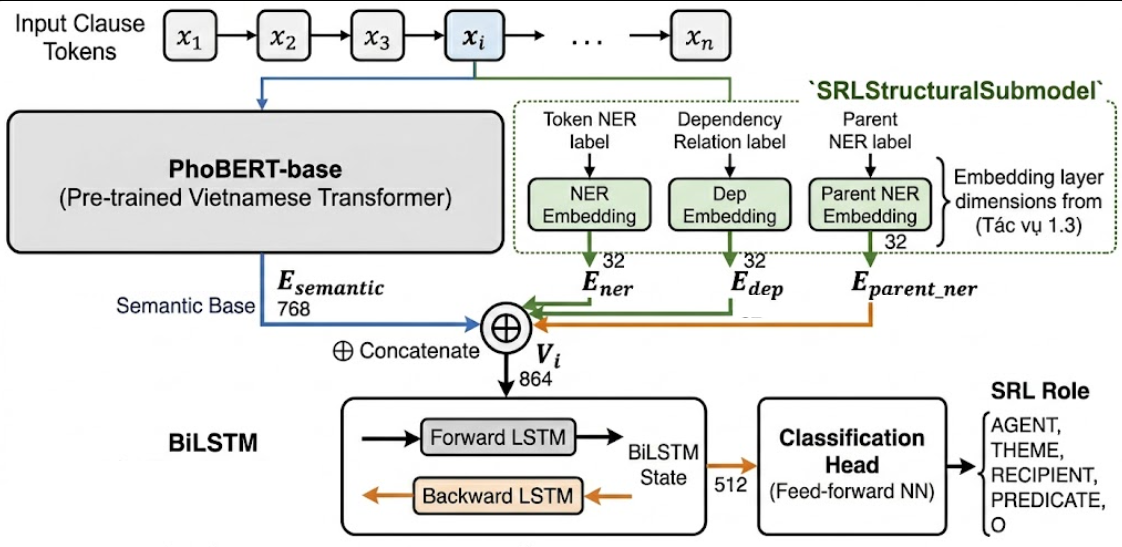
\includegraphics[width=1.0\textwidth]{Image/srl_model.png}
    \caption{Sơ đồ kiến trúc JointSRLModel: Kết hợp Semantic Base, Structural Embeddings và lớp Sequential Modeling.}
    \label{fig:joint_srl_arch}
\end{figure}

Hệ thống vector đầu vào cho mỗi token $x_i$ là một vector tổng hợp $V_i$:
\begin{equation}
V_i = [E_{semantic} \oplus E_{ner} \oplus E_{dep} \oplus E_{parent\_ner}]
\end{equation}

Trong đó:
\begin{enumerate}
    \item \textbf{Semantic Base ($E_{semantic}$)}: Trích xuất từ tầng ẩn cuối cùng của PhoBERT ($768$ chiều). Vector này mang thông tin ngữ cảnh đa chiều, giúp model hiểu nghĩa của từ trong mối tương quan với các từ xung quanh.
    \item \textbf{Structural Embeddings ($E_{ner}, E_{dep}, E_{parent\_ner}$)}: 
    Để tối ưu hóa, hệ thống không đưa các nhãn nhị phân (one-hot) mà thông qua một mạng con \texttt{SRLStructuralSubmodel}. Mạng này ánh xạ các thực thể và quan hệ cú pháp vào một không gian nhúng thấp chiều ($32$ chiều mỗi loại):
    \begin{itemize}
        \item \textbf{Token NER ($E_{ner}$)}: Cung cấp "manh mối" về loại thực thể. Một token là \texttt{PARTY} sẽ có xác suất cao là \texttt{AGENT} (người thực hiện) hoặc \texttt{RECIPIENT} (người thụ hưởng).
        \item \textbf{Dependency Relation ($E_{dep}$)}: Nhãn quan hệ phụ thuộc (như \textit{nsubj, obj, obl}). Ví dụ, một từ có quan hệ \textit{nsubj} với động từ chính gần như chắc chắn đóng vai trò \texttt{AGENT}.
        \item \textbf{Parent NER ($E_{parent\_ner}$)}: Đây là đặc trưng "vượt cấp" độc đáo. Bằng cách nhìn vào nhãn thực thể của từ "cha" (Head word) trong cây cú pháp, model có thể hiểu được phân cấp ngữ nghĩa. Nếu từ cha là một \texttt{PREDICATE} (động từ pháp lý), từ con mang nhãn \texttt{MONEY} sẽ đóng vai trò là \texttt{THEME} (đối tượng giao dịch).
    \end{itemize}
    \item \textbf{Sequential Modeling (BiLSTM)}: 
    Sau khi kết hợp các vector ($768 + 32 \times 3 = 864$ chiều), chuỗi được đưa qua lớp \textbf{BiLSTM} hai chiều với $256$ unit mỗi chiều (tổng $512$). 
    \begin{itemize}
        \item \textit{Forward LSTM}: Nắm bắt thông tin tiền ngữ cảnh.
        \item \textit{Backward LSTM}: Nắm bắt thông tin hậu ngữ cảnh.
    \end{itemize}
    Lớp này đóng vai trò "hòa trộn" giữa tri thức tĩnh (nhãn cấu trúc) và tri thức động (ngữ nghĩa PhoBERT) để đưa ra quyết định cuối cùng về vai trò ngữ nghĩa của token trong dòng chảy của mệnh đề.
\end{enumerate}

\paragraph{Điểm lợi của phương pháp:} 
Việc bổ sung \texttt{Structural Embeddings} đóng vai trò như một cơ chế "Shortcut" (đường tắt). Thay vì bắt PhoBERT phải tự học lại các quy tắc cú pháp phức tạp từ đầu (đòi hỏi dữ liệu cực lớn), chúng ta trực tiếp "tiêm" tri thức ngôn ngữ học vào model. Điều này đặc biệt hiệu quả trong miền dữ liệu hẹp như hợp đồng pháp lý, giúp model đạt độ chính xác cao ngay cả với tập dữ liệu huấn luyện giới hạn.

\paragraph{Mô tả thuật toán xử lý đặc trưng (Inference):}
Hệ thống sử dụng kỹ thuật "Mặt nạ nhãn ký tự" (Character Label Mask) để đảm bảo kết quả trích xuất SRL khớp hoàn toàn với văn bản gốc dù có sự sai lệch giữa tokenizer của Stanza và PhoBERT.

\begin{verbatim}
Algorithm: SRL Character Masking
Input: Predicted SRL labels per token, Original Text, NER Entities
Output: Predicate and Arguments dictionary

1. char_mask = Array of length(Original Text), initialized to None
2. For each entity in NER:
      If entity.label == "PREDICATE":
         Fill char_mask[span] with "PREDICATE"
3. For each token i and its predicted label L:
      Map token i to real_start, real_end in Original Text
      For idx from real_start to real_end:
         If char_mask[idx] is None: char_mask[idx] = L
4. current_role = None, buffer = ""
5. For idx, label in char_mask:
      If label != current_role:
         Flush buffer to results[current_role]
         current_role = label, buffer = char_at(idx)
      Else:
         buffer += char_at(idx)
6. Return results
\end{verbatim}

\paragraph{Ví dụ trực quan:}
\begin{itemize}
    \item \textbf{Mệnh đề}: "Bên A bàn giao vật tư cho bên B."
    \item \textbf{Trích xuất}:
    \begin{itemize}
        \item \texttt{Predicate}: "bàn giao"
        \item \texttt{Agent}: "Bên A"
        \item \texttt{Theme}: "vật tư"
        \item \texttt{Recipient}: "cho bên B"
    \end{itemize}
\end{itemize}

\subsubsection{Phân loại ý định mệnh đề (Task 2.3)}

Tác vụ này xác định chức năng pháp lý của toàn bộ mệnh đề.

\paragraph{Lược đồ ý định (Intents):}
\begin{itemize}
    \item \textbf{Obligation}: Nghĩa vụ bắt buộc thực hiện (từ khóa: "phải", "có trách nhiệm").
    \item \textbf{Prohibition}: Hành vi bị cấm (từ khóa: "không được", "cấm").
    \item \textbf{Right}: Quyền lợi của một bên (từ khóa: "có quyền", "được phép").
    \item \textbf{Termination Condition}: Điều kiện chấm dứt hợp đồng.
    \item \textbf{Other}: Các câu thông tin chung hoặc định nghĩa.
\end{itemize}

\paragraph{Pipeline phân loại đa tầng (Fallback Strategy):}
Vì các hợp đồng pháp lý yêu cầu độ chính xác tuyệt đối, hệ thống được thiết kế theo kiến trúc "phòng ngự nhiều lớp" (Defense-in-depth) thông qua hàm \texttt{classify\_intent} trong tệp \texttt{intent\_classifier.py}. Hệ thống sẽ tuần tự thử nghiệm các mô hình từ độ phức tạp cao đến thấp, đảm bảo luôn có kết quả ngay cả khi gặp lỗi ngoại lệ (exception) hay thiếu hụt tài nguyên (OOM).

\begin{enumerate}
    \item \textbf{Lớp 1 - Robust Transformer (PhoBERT):} Đây là lõi suy luận chính. Cụm văn bản được tách từ (tokenize) bằng thuật toán BPE và đưa vào \texttt{RobustIntentModel}. Nhờ cơ chế Self-Attention, lớp này có khả năng nắm bắt "ý định ngầm" (implicit intent). Ví dụ, câu \textit{"Bên A sẽ thanh toán tiền cọc"} không có từ khóa "nghĩa vụ" rõ ràng, nhưng PhoBERT vẫn phân loại chính xác là \texttt{Obligation} nhờ học được ngữ cảnh khái quát từ hàng ngàn mẫu huấn luyện.
    \item \textbf{Lớp 2 - ML Baseline (TF-IDF + Logistic Regression):} Nếu Lớp 1 thất bại (ví dụ: mô hình chưa được tải vào VRAM), hệ thống sẽ kích hoạt Lớp 2. Tại đây, câu văn được chuyển đổi thành một ma trận thưa (sparse matrix) thông qua \texttt{TfidfVectorizer} với dải n-gram $(1, 2)$. Thuật toán Logistic Regression sau đó sẽ tính toán xác suất $\sigma(W^T \cdot X + b)$ để gán nhãn. Mặc dù không hiểu được thứ tự từ vựng phức tạp, mô hình học máy truyền thống này hoạt động cực kỳ nhanh và nhẹ.
    \item \textbf{Lớp 3 - Rule-based Matching:} Trong kịch bản xấu nhất khi cả hai mô hình AI đều không khả dụng, hệ thống rơi về cơ chế quét từ khóa thuần túy (Heuristic). Thuật toán duyệt qua một từ điển được định nghĩa sẵn (\texttt{INTENT\_KEYWORDS}). Nếu trong câu có chứa cụm "không được phép" hoặc "cấm", nó lập tức trả về \texttt{Prohibition}. Nếu không khớp bất kỳ luật nào, hệ thống gán nhãn an toàn là \texttt{Other}.
\end{enumerate}

\paragraph{Thiết kế Head phân loại và Multi-Sample Dropout:}
Mô hình \texttt{RobustIntentModel} được xây dựng bằng cách kế thừa kiến trúc \texttt{RobertaForSequenceClassification} (nền tảng của PhoBERT) và tích hợp thêm lớp bọc xử lý nhiễu. Điểm cốt lõi của thiết kế này nằm ở việc tối ưu hóa vector đại diện ngữ cảnh (Context Representation) thông qua cơ chế lan truyền song song.

Mặc dù ma trận trạng thái ẩn cuối cùng trả về có kích thước $\mathbf{H} \in \mathbb{R}^{L \times D}$ (với $L$ là độ dài chuỗi, $D=768$), nhưng theo đặc thù của dòng RoBERTa, lớp \texttt{classifier} (\texttt{RobertaClassificationHead}) sẽ thực hiện trích xuất vector tại vị trí token đặc biệt đầu tiên $h_{<s>} \in \mathbb{R}^{D}$. Vector này được coi là "tổng hòa ngữ nghĩa" của toàn bộ mệnh đề nhờ cơ chế Self-Attention.

Để gia tăng khả năng tổng quát hóa trên tập dữ liệu pháp lý nhỏ, lớp bọc \texttt{MultiSampleDropoutWrapper} triển khai kỹ thuật \textbf{Multi-Sample Dropout} \autocite{multidrop}. Thay vì sử dụng một tầng Dropout đơn lẻ, hệ thống tạo ra $K = 5$ nhánh xử lý song song. Thuật toán chi tiết như sau:

\begin{enumerate}
    \item \textbf{Forward Pass:} Vector trạng thái ẩn $\mathbf{H}$ từ PhoBERT được đưa vào module \texttt{MultiSampleDropout}.
    \item \textbf{Parallel Dropout:} Hệ thống áp dụng 5 mặt nạ Dropout khác nhau $M_1, \dots, M_5$ với xác suất loại bỏ ($p$) tăng dần từ $0.1$ đến $0.5$ lên cùng một đầu vào $\mathbf{H}$.
    \item \textbf{Shared Classification:} Cả 5 phiên bản sau Dropout đều được đưa qua cùng một lớp \texttt{classifier} (bao gồm một tầng Dense kết hợp hàm kích hoạt Tanh và tầng Linear cuối cùng).
    \item \textbf{Aggregation:} Logits cuối cùng là trung bình cộng của 5 kết quả đầu ra, giúp triệt tiêu các sai số ngẫu nhiên:
    \begin{equation}
    Z_{final} = \frac{1}{5} \sum_{k=1}^{5} \text{Classifier}(\text{Dropout}_k(\mathbf{H}))
    \end{equation}
\end{enumerate}

Việc áp dụng nhiều mức Dropout khác nhau trong cùng một lần huấn luyện giúp mô hình không bị phụ thuộc quá mức vào bất kỳ nhóm neuron cụ thể nào, từ đó nhận diện ý định pháp lý (như \texttt{Obligation} hay \texttt{Prohibition}) dựa trên các đặc trưng bền vững nhất.

\begin{figure}[H]
    \centering
    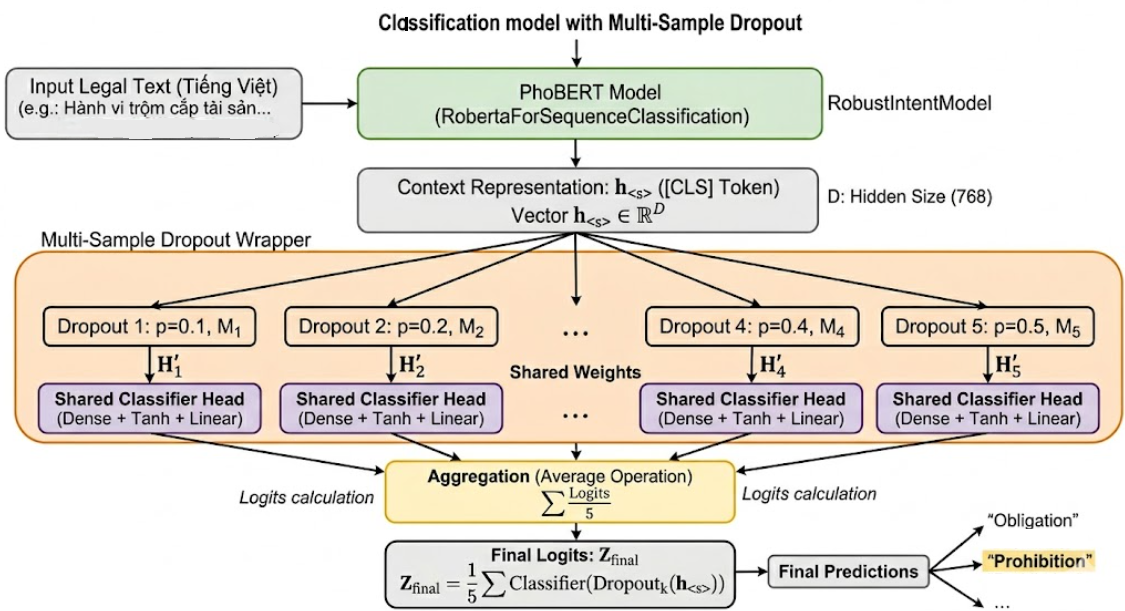
\includegraphics[width=1.0\textwidth]{Image/intent_model.png}
    \caption{Sơ đồ kiến trúc mô hình phân loại với cơ chế Multi-Sample Dropout can thiệp vào Classification Head.}
    \label{fig:intent_arch}
\end{figure}